\documentclass[11pt,a4paper]{article}
\usepackage[utf8]{inputenc}
\usepackage{amsmath}
\usepackage[toc,page]{appendix}
\usepackage{xcolor}
\numberwithin{equation}{section}
\numberwithin{table}{section}
\numberwithin{figure}{section}
\usepackage{amsfonts}
\usepackage{float}
\usepackage{amssymb}
\usepackage{bbm}
\usepackage{amsthm}
\usepackage{cite}
\usepackage{hyperref}
\usepackage{setspace}
\usepackage{array}
\usepackage{graphicx}
\usepackage{tabularx}
\usepackage[german]{babel}
\usepackage{pdfpages}
\addto\captionsgerman{
  \renewcommand{\figurename}{Abb.}
  \renewcommand{\tablename}{Tab.}
}
\newtheorem{satz}{Theorem}[section]
\newtheorem{lemma}[satz]{Lemma}
\newtheorem{aussage}[satz]{Aussage}
\newtheorem{korollar}[satz]{Corollary}
\newtheorem{definition}[satz]{Definition}
\newtheorem{bemerkung}[satz]{Bemerkung}
\newtheorem{proposition}[satz]{Proposition}
\newtheorem{example}[satz]{Beispiel}
\newtheorem{notation}[satz]{Notation}
\newtheorem{uberblick}[satz]{Overview}
\newtheorem{vermutung}[satz]{Conjecture}
\usepackage[left=2.5cm,right=2.5cm,top=2.5cm,bottom=2cm]{geometry}
\author{Linus Rumpel und Florian Brütsch}
\title{Schachbrett trifft Graphentheorie!}
\begin{document}
\vspace*{2em}
\begin{center} \Huge \bf
Schachbrett trifft Graphentheorie! \\ 
\Large
Landeswettbewerb Balingen\\
\begin{center}

\includegraphics[scale=0.6]{00.jpg} 
\end{center}

\huge
Schüler experimentieren 2021 \vspace*{1em}\\
\end{center}
\thispagestyle{empty}
~ 
\begin{center}
\includegraphics[scale=0.5]{Schüler Experimentieren Bild.jpg}\\
\tiny{*Fotomontage}\\
\vspace*{4em}
 \Large 
Florian Brütsch, Otto-Hahn-Gymnasium, Tuttlingen, Klasse 9\\
Linus Rumpel, Otto-Hahn-Gymnasium, Tuttlingen, Klasse 9\\
Schülerforschungszentrum SFZ in Tuttlingen \\
\vspace{1em}
\large
März 2021
\end{center}

\clearpage
\tableofcontents
\listoffigures

~
\thispagestyle{empty}
\clearpage


\section{Einführung}
\setcounter{page}{1}
\subsection{Einleitung}
Vor einem Jahr haben wir beim Schachspielen gemerkt, dass es ein enormer Zufall ist, dass jedes
weiße Feld nur an schwarze grenzen und umgekehrt.\par \noindent
Wenn nur ein Feld anders gefärbt wäre, würde dies nicht der Fall sein. Dann bilden sich (größere) schwarze und weiße Bereiche, welche wir Gebiete nennen.  Wir haben uns daher gefragt, wie viele Gebiete eigentlich im Schnitt herauskommen, wenn man jedes Feld stattdessen völlig zufällig färbt.\begin{figure}[H]\label{bild1}
\begin{center}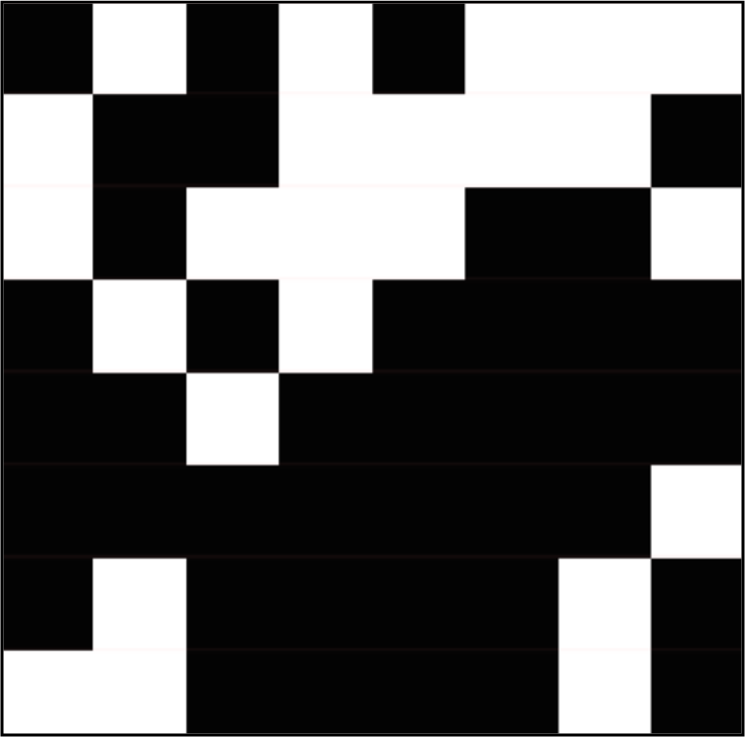
\includegraphics[scale=0.10]{1.png}
\caption{Beispielfärbung.}\end{center}
\end{figure}
\par\noindent Dies hat uns zu mathematischen Objekten wie Graphen und Erwartungswerten und am Ende zu einer Abschätzung der sich im Mittel ergebenden Gebiete geführt. Schließlich haben wir unser Wissen auf andere geometrische Anordnungen übertragen (Tori, Waben, höhere Dimensionen).
Um die Güte unserer Abschätzungen überprüfen zu können, haben wir dies anhand einiger numerischer Simulationen bestätigt. Unter anderem haben wir den Erwartungswert für kleine Felder direkt berechnet.  


\subsection{Grundidee}
Die Grundidee besteht darin, das Schachbrett als Graph darzustellen. Ein Graph ist hierbei eine Ansammlung von einer gewissen Menge an (gefärbten) Punkten $P$, die mit Linien (bzw. Kanten) $L$ verbunden werden oder nicht (vgl. \cite{graph}). In unserem Fall entspricht jedes Feld dabei einem Punkt, also entsprechend schwarz oder weiß. Zwei Punkte werden dabei durch eine Linie verbunden, falls die zugehörigen Felder aneinander grenzen (waagrecht und senkrecht) und gleichfarbig sind.  Zum Beispiel:\begin{center}
\begin{figure}[H]\label{bild2}
\begin{center}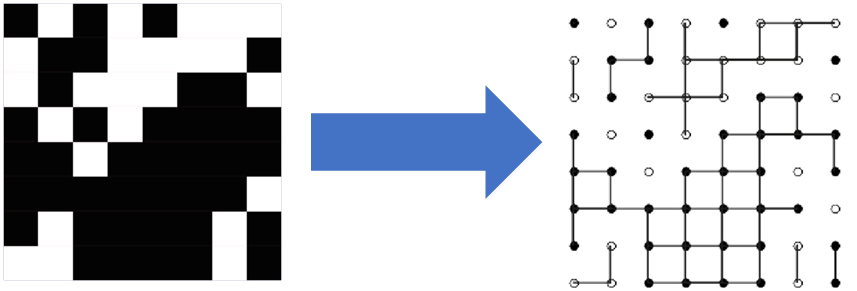
\includegraphics[scale=0.5]{2.png}
\caption{Darstellung der Färbung als Graph.}\end{center}
\end{figure}
\end{center}
Mathematisch heißt dies, dass der gesuchte Wert der Anzahl der Gebiete $G$ oder der Zusammenhangskomponenten (vgl. \cite{zusammenhangskomponente}) des Graphen entspricht. Im obigen Beispiel wären das 17. \par\noindent


\section{Formeln}
In diesem Modell wollen wir nun eine allgemeine Formel aufstellen, bei der wir die Anzahl der Gebiete im Mittel abschätzen wollen, da eine exakte Formel im Allgemeinen nicht möglich sein wird, weil es auch für Zusammenhangskomponenten keine gibt.  Hierfür benutzen wir den Erwartungswert $E(A)$ für ein Ergebnis eines Zufallsexperiments (Zufallsvariable) $A$ (vgl. \cite[S. 133]{mathe09}). Das Nützliche dabei ist, dass diese Formel schließlich für einen praktisch beliebigen Graphen gilt. Sie ergibt sich, indem wir geschickt Punkte, Kanten und geschlossene kleinere Einheiten, meist Quadrate, zählen. Später wenden wir diese Formel auf verschiedene geometrische Objekte an. 
\subsection{Allgemeine Formel}

Wir führen ein paar Variablen ein:
\begin{itemize}
\item Sei $P$ die Anzahl der Punkte,
\item  $L$ die Anzahl der Linien
\item  und $G$ die Anzahl der Gebiete oder auch Zusammenhangskomponenten (unabhängig von der Farbe).
\end{itemize}
Nun gilt: 
\begin{aussage} 
Die Anzahl der Gebiete ist niemals kleiner als die Differenz aus Punkten und Linien oder genauer:
$$G\geq P-L.$$
\end{aussage}
\begin{proof}
Dies lässt sich wie folgt sehen:\par\noindent
Falls $L=0$, so gilt offensichtlich $G=P$, da keine Punkte miteinander verbunden sind. Es gibt also gleich viele Punkte wie Gebiete.\par\noindent
Nun verbindet jede Linie, die neu dazukommt, entweder 2 Gebiete, die noch nicht miteinander verbunden waren, oder eben nicht. Also kann mit jeder neuen Linie die Anzahl der Gebiete $G$ nur um eins kleiner werden oder gleich bleiben. Im Extremfall wird sie also jedes Mal um eins kleiner. Also ist $G$ sicherlich größer gleich $P-L$.
\end{proof} \par\noindent
Diese Formel lässt sich jedoch noch verbessern. Vergleiche: \par\noindent 
\begin{minipage}{0.4\textwidth}
\begin{figure}[H]\label{bild3}
\begin{center}
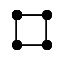
\includegraphics[scale=1]{3}
\caption{Quadrat.}
\end{center}
\end{figure} 
\end{minipage}
\begin{minipage}{0.2\textwidth}
und
\end{minipage}
\begin{minipage}{0.4\textwidth}
\begin{figure}[H]\label{bild4}
\begin{center}
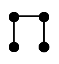
\includegraphics[scale=1]{4}
\caption{Quadrat mit gel. Kante.}
\end{center}
\end{figure} 
\end{minipage}
\par\noindent 
Es fällt auf, dass beide Graphen gleich viele Zusammenhangskomponenten haben. Wir dürfen also aus jedem vorkommenden Quadrat (damit meinen wir immer nur kleine $2\times 2$-Quadrate!) die untere Linie löschen, ohne die Anzahl an Zusammenhangskomponenten zu verändern. Wir nennen die Anzahl von vorkommenden Quadraten im Graphen $Q$. \newpage
In unserem Beispiel sieht das dann so aus:
\begin{center} 
\begin{figure}[H]\label{bild11}
\begin{center}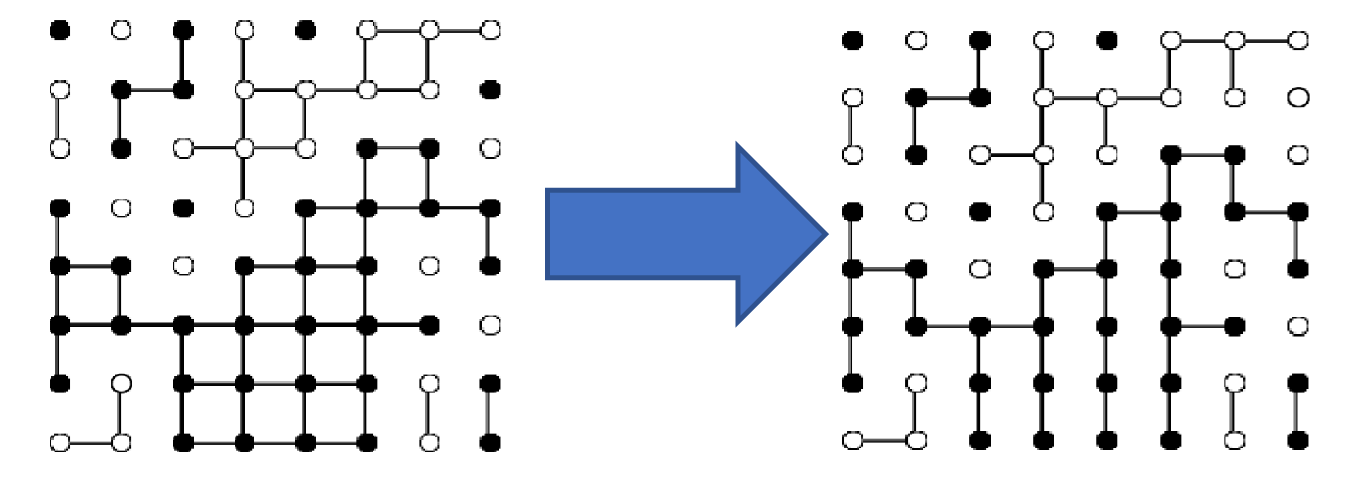
\includegraphics[scale=0.3]{11}
\caption{Kanten aus Quadraten löschen.}\end{center}
\end{figure}
\end{center}
Damit definieren wir zu unserem Graphen einen zugehörigen bearbeiteten Graphen, wobei wir dazu aus jedem Quadrat die untere Kante löschen. Seien nun $P', L'$, $G'$ die Anzahl der Punkte, Linien und Gebiete im bearbeiteten Graphen.
Es gilt $G=G'$ aber $L'=L-Q$ und $P=P'$. Damit lässt sich folgende Aussage zeigen:
\begin{aussage}
Unsere Formel lässt sich zu $E(G)\geq P-E(L)+E(Q)$ verbessern.
\end{aussage}
\begin{proof}
Es gilt $E(G)=E(G')\geq E(P'-L')=E(P-L+Q)$ Da der Erwartungswert die Eigenschaft $E(A+B)=E(A)+E(B)$ für zwei Zufallsvariablen $A$ und $B$ erfüllt, folgt damit $$ E(G)\geq E(P)-E(L)+E(Q).$$ Nun hängt die Anzahl der Punkte gar nicht von der Wahl der zufälligen Färbung ab. 
Also gilt $E(P)=P$ und wir landen bei unserer Aussage:
$$\boxed{E(G)\geq P-E(L)+E(Q).}$$
\end{proof}
\par\noindent Das Schöne an der Formel ist, dass sie grundsätzlich nicht nur fürs Schachbrett gilt, sondern auch für alle anderen Formen, Tori und Dimensionen. Dabei müssen wir unter einem Quadrat im Allgemeinen eine Form verstehen, aus welcher man immer etwas löschen darf (siehe unten).
\subsection{Anwendungen der Abschätzung auf konkrete Muster}
\subsubsection{Schachbrett}
Betrachten wir nun die Formel $E(G)\geq P-E(L)+E(Q)$. Dann setzen wir die Angaben eines Schachbrettes mit der Größe $m\cdot n$ ein.\par\noindent
$P$ ist die Anzahl der Punkte, beim Schachbrett sind das $m\cdot n$.
$E(L)$ ist der Erwartungswert der Kanten (Linien), also die Anzahl aller möglichen Kanten mal die Wahrscheinlichkeit, dass eine einzelne Linie existiert (d.h. 1/2). Da $m\cdot(n-1)+(m-1)\cdot n$ Kanten möglich sind, entspricht dieser Teil insgesamt:
$$E(L)=\frac{1}{2}(m(n-1)+(m-1)n)$$ \par \noindent
Bei $E(Q)$ verfahren wir gleich und multiplizieren die Anzahl der möglichen Quadrate
$ (m-1)\cdot(n-1)$ mit der Wahrscheinlichkeit, dass ein beliebiges dieser Quadrate vorhanden ist. Diese Wahrscheinlichkeit ist 1/8, da es 16 verschiedene Möglichkeiten gibt, die Eckpunkte eines potentiellen Quadrates zu färben und in 2 von diesen Fällen ein Quadrat existiert. \par\noindent
Also insgesamt: 
$$E(Q)=\frac{1}{8}(m-1)\cdot(n-1)$$
Fügen wir nun alle gesammelten Teile zusammen, entsteht folgender Term:
\begin{align*}
E(G)&\geq m\cdot n-\frac{1}{2} (m\cdot(n-1)+(m-1)\cdot n)+\frac{1}{8} (m-1)\cdot(n-1)  \\
&=\frac{1}{8} m\cdot n+\frac{1}{2} (m+ n)-\frac{1}{8}(m+n)+\frac{1}{8}\\
&\Rightarrow E(G)\geq \frac{1}{8} m \cdot n+\frac{3}{8}(m+n)+\frac{1}{8}=\frac{mn+3(m+n)+1}{8}
\end{align*}
Für das reguläre Schachbrett $(m=n=8)$ ergibt sich also ein Wert von $$E(G)\geq \frac{64+3\cdot 16+1}{8}=14,125$$
\subsubsection{Formel bei einem Torus-Schachbrett}
Ein weiterer interessanter Gedanke ist die Vorstellung, dass sich gegenüberliegende Randfelder auf dem Schachbrett trotzdem berühren. Sozusagen rollen wir unser Brett also erst zu einem Zylinder zusammen und dann diesen Zylinder zu einer Art Donut. In der Mathemetik nennt man dieses Objekt dann einen Torus (vgl. \cite{torus}).\par\noindent
Auch hiervon lässt sich der Erwartungswert bestimmen.\par\noindent
Zunächst die Punkte: Da ein Schachbrett-Torus gleich viele Punkte wie das Schachbrett hat, gilt auch hier $P=m\cdot n$ .\par\noindent
Auch die Kanten sind ähnlich, allerdings kommt noch die Verbindungskante von ganz rechts nach ganz links hinzu (analog oben/unten). Also wird beispielsweise aus $m(n-1)$ nun $m\cdot(n-1+1)=mn$. Dementsprechend gilt
$$L=mn+mn=2mn.$$
Wie bei den Kanten kann man auch bei den Quadraten einiges vom Schachbrett "ubernehmen. So ändert sich auch die Anzahl der möglichen Quadrate nur in so fern, dass pro Dimension nur eine Reihe bzw. Spalte möglicher Quadrate hinzukommt. Die Formel wird also statt $(m-1)\cdot(n-1)$  zu $Q=m\cdot n$.\par\noindent
Wenn wir diese Terme nun gemeinsam mit den zugehörigen Wahrscheinlichkeiten zusammenfügen, entsteht der folgende Term:
\begin{align*}
E(G)\geq P-E(L)+E(Q)&=mn-\frac{1}{2}(2mn)+\frac{1}{8}mn=mn-mn+\frac{1}{8}mn =\frac{1}{8}mn
\end{align*}

\subsubsection{Formel bei mehreren Farben fürs Schachbrett}
Bisher haben wir stets nur zwei Farben betrachtet. Möchten wir uns stattdessen mehr wie zwei Farben anschauen, muss man nur die Wahrscheinlichkeiten für einzelne Linien/Quadrate ändern. Dazu fügt man für die Anzahl der Farben die Variable $F$ ein.\par\noindent
Die Wahrscheinlichkeit, dass eine Kante in einer bestimmten Farbe da ist, liegt bei $$\frac{F}{F^2}=\frac{1}{F}$$
Die Wahrscheinlichkeit, dass ein Quadrat in einer Farbe existiert, liegt hingegen bei
$$\frac{F}{F^4}=\frac{1}{F^3}$$
Denn es gibt $F^4$  Möglichkeiten für die Farben in einem Quadrat. $F$ davon sind gleichfarbig. 
Wenn wir diese Werte in die Formel einsetzten, kommen wir auf folgende Formel: 
\begin{align*}
E(G)&\geq m\cdot n-\frac{1}{F}(m\cdot(n-1)+(m-1)\cdot n)+\frac{1}{F^3}(m-1)\cdot(n-1)\\
&=\left(1-\frac{2}{F}+\frac{1}{F^3}\right)mn+\left(\frac{1}{F}-\frac{1}{F^3}\right)(m+n)+\frac{1}{F^3}\\
\Rightarrow E(G)&\geq\left(1-\frac{2}{F}+\frac{1}{F^3}\right)mn+\left(\frac{1}{F}-\frac{1}{F^3}\right)(m+n)+\frac{1}{F^3}
\end{align*}
Für drei Farben gilt also beispielsweise:
$$E(G)\geq\left(\frac{10}{27} \right)mn+\left(\frac{8}{27}\right)(m+n)+\frac{1}{27}$$
Auch für den Torus lässt sich auf diese Weise eine Formel für beliebig viele Farben herleiten. Wir erinnern an die Formel für zwei Farben:
$$E(G)\geq mn-\frac{1}{2}(2mn)+\frac{1}{8}mn.$$
Ersetzt man wieder $\frac{1}{2}$ durch $\frac{1}{F}$ und $\frac{1}{8}$ durch $\frac{1}{F^3}$ so ergibt sich:
$$E(G) \geq mn-\frac{1}{F}(2mn)+\frac{1}{F^3}mn=mn\left(1-\frac{2}{F}+\frac{1}{F^3}\right)=mn\left(\frac{F^3-2F^2-1}{F^3}\right)$$
\subsection{Erwartungswert beim Quader}

Ein weiterer interessanter Gedanke ist die Vorstellung, dass wir unser Problem in einer Dimension höher betrachten. Dann handelt es sich nicht um ein Schachbrett, sondern um einen Quader.

\noindent\begin{minipage}{0.6\textwidth}
\noindent Auch hier lässt sich der Erwartungswert abschätzen. Wir benutzen nun die Variablen $m$, $n$ und $o$ für die Größe des Quaders. Hierbei betrachten wir zunächst den Fall mit zwei Farben.\par\noindent
Nun setzen wir die Variablen in unsere Formel ein:
$$E(G)\geq P-E(L)+E(Q)$$
Die Anzahl der Punkte lässt sich leicht herleiten:
$$P=m\cdot n\cdot o$$
\\
\end{minipage}
\begin{minipage}{0.4\textwidth}
\begin{figure}[H]\label{bild5}
\begin{center}
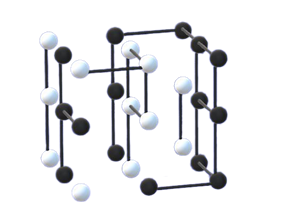
\includegraphics[scale=0.7]{Bild267.png}
\caption{Graph eines Quaders.}
\end{center}
\end{figure} 
\end{minipage}
Der Erwartungswert der Linien ist wieder die Wahrscheinlichkeit, dass eine Linie existiert mal die Anzahl der möglichen Linien. \par\noindent
Also  
$$E(L)=\frac{1}{2}[(m-1)no+(n-1)mo+(o-1)mn].$$
Bei den Quadraten müssen wir jetzt jedoch aufpassen:
\vspace{-2em}
\begin{center}
\begin{figure}[H]\label{bild6}
\begin{center}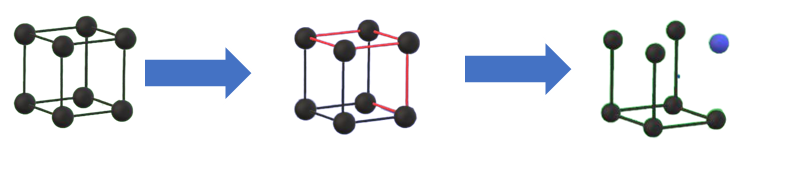
\includegraphics[scale=0.9]{6.png}
\caption{Löschen Quader; falsch.}\end{center}
\end{figure}
\end{center}
Dies sieht man sehr gut an diesem Beispiel. Aus dem ersten Graphen wird pro Quadrat eine (die rote) Kante gelöscht (Pfeil 1). Wie man im dritten Bild erkennen kann, ist der blaue Teil dann von den anderen abgetrennt.\par
\noindent
Stattdessen betrachten wir das Objekt aus einer festen Richtung. Wir löschen aus jedem vollständigen Quadrat die Kante, die uns am nächsten liegt. Bei den Quadraten, bei denen alle Kanten von uns gleich weit entfernt sind, löschen wir keine Kante. So ist klar, dass wir nichts doppelt löschen. Also bleiben die Quadrate, die in einer bestimmten Richtung liegen unverändert:
\begin{center}
\begin{figure}[H]\label{bild6b}
\begin{center}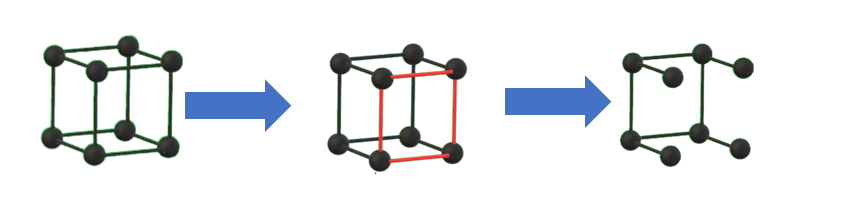
\includegraphics[scale=0.8]{6b.PNG}
\caption{Löschen Quader; korrekt.}\end{center}
\end{figure}
\end{center}
Wir bezeichnen mit $Q$ also jetzt nur noch die Anzahl von Quadraten, aus denen wir löschen dürfen. 
Die Formel ist also
 $$E(Q)=\frac{1}{8}(m-1)(n-1)o+\frac{1}{8}(m-1)(o-1)n$$ Der dritte Term, den man eigentlich erwarten würde (d.h. $\frac{1}{8}m(n-1)(o-1)$) fehlt aus dem oben genannten Grund, nachdem die  Quadrate in der dritten Raumebene ignoriert werden müssen. 
Fügen wir nun diese Terme zusammen, ergibt sich:\small
\begin{align*}
E(G)&\geq mno-\frac{1}{2} [mno-no+mno-mo+mno-mn]\\
&\phantom{blablablablablabablablabla}+\frac{1}{8} (m-1)(n-1)o+\frac{1}{8} (m-1)(o-1)n\\
&=mno-\frac{1}{2} [3mno-no-mo-mn]+\frac{1}{8} (m-1)(n-1)o+\frac{1}{8} (m-1)(o-1)n\\
&=[-\frac{1}{2} mno+\frac{1}{2} no+\frac{1}{2} mo+\frac{1}{2} mn]+\frac{1}{8} mno-\frac{1}{8} no\\
&\phantom{blablablabblablalblablabla}+\frac{1}{8} o-\frac{1}{8} mo+\frac{1}{8} mno-\frac{1}{8} no+\frac{1}{8} n-\frac{1}{8} mn\\
&=-\frac{1}{4} mno+\frac{1}{4} no+\frac{3}{8} mo+\frac{3}{8} mn+\frac{1}{8} o+\frac{1}{8} n
\end{align*}\normalsize
Leider ist der obige Term in sehr vielen Fällen negativ (z.B. für $m=n=o=8$), so dass er in diesen Fällen unbrauchbar ist, da der Erwartungswert immer größer gleich eins ist. Dies ist so, da es immer mindestens ein Gebiet gibt. \par\noindent

\noindent Für stabförmige Körper hingegen (z.B. $m=2,~ n\geq 5,~ o=3$) liefert die Formel dennoch einen Wert über eins und somit zumindest eine Abschätzung mit tatsächlich nützlicher Aussage. \par\noindent
Für mehrere Farben wird die Formel tendenziell brauchbarer. Dies ist anschaulich klar, da mehr Farben automatisch bedeuten, dass gleichfarbige Felder seltener aneinandergrenzen. Somit werden die Gebiete automatisch kleiner und deren Anzahl somit größer. In unserer Formel ersetzen wir dabei wieder $\frac{1}{2}$ durch $\frac{1}{F}$ und $\frac{1}{8}$ durch $\frac{1}{F^3}$. Dann ergibt sich:\small
\begin{align*}
E(G)&\geq mno-\frac{1}{F} [mno-no+mno-mo+mno-mn]+\frac{1}{F^3} (m-1)\cdot(n-1)o\\
&\phantom{blablablablablablablablabla}+\frac{1}{F^3} (m-1)\cdot(o-1)n\\
&=\left(1-\frac{3}{F}+\frac{2}{F^3} \right)mno+\left(\frac{1}{F}-\frac{2}{F^3 }\right)no+\left(\frac{1}{F}-\frac{1}{F^3 }\right)mo\\
&\phantom{blablblablablaablabla}+\left(\frac{1}{F}-\frac{1}{F^3 }\right)mn+\frac{1}{F^3}o+\frac{1}{F^3}n
\end{align*}
\normalsize
Es fällt auf, dass bereits für $F=3$ immer ein positiver Wert übrig bleibt, nämlich:
$$\frac{2}{27} mno+\frac{7}{27}no+\frac{8}{27}(mo+mn)+\frac{1}{27}(o+n)$$
Für den $8\times 8\times 8$ Würfel mit drei Farben ergibt sich also eine untere Schranke von 
$$E(G) \geq \frac{1024+23\cdot64+16}{27}=\frac{2512}{27}=93,037$$
Für $F=4$ ergibt sich $E(G) \geq 188,25$
\subsubsection{Torus Quader}
Besonders interessant ist die Betrachtung des Würfels als Torus. Dies lässt sich zwar nur schwer vorstellen, da man hier die vierte Dimension zur Veranschaulichung bräuchte, trotzdem lässt sich davon der Erwartungswert bestimmen. Wir berechnen dies gleich für beliebig viele Farben, da für zwei Farben wegen den zusätzlichen Verbindungen ohnehin mit einem noch schlechteren Wert zu rechnen ist. \par\noindent
Die Anzahl der Punkte ist wie beim Quader 
$$P=m\cdot n\cdot o$$
Die Anzahl der Kanten ist anders als beim Würfel, da ja wieder die weiteren Verbindungskanten hinzukommen. 
Die Formel ist also 
$$E(L)=\frac{1}{F} [mno+mno+mno]=\frac{3}{F}mno $$
Für die Quadrate erhält man aus denselben Gründen
$$E(Q)=\frac{1}{F^3}(2mno)=\frac{2}{F^3}mno $$
Fügen wir die Terme wieder zusammen, so erhalten wir
$$E(G)\geq\left(1-\frac{3}{F}+\frac{2}{F^3}\right)mno $$
Für $F=3$ bleibt also wieder etwas übrig. Hierbei sind die Werte für den $8\times8\times8$ Torus dementsprechend $\frac{1024}{27}\approx 37,92$ für $F=3$ und $144$ für $F=4$.
\subsection{Sechseckschachbrett}
Auch interessant wäre, wenn die einzelnen Felder des Schachbretts Sechsecke wären. 
\begin{center}
\begin{figure}[H]\label{bild7}
\begin{center}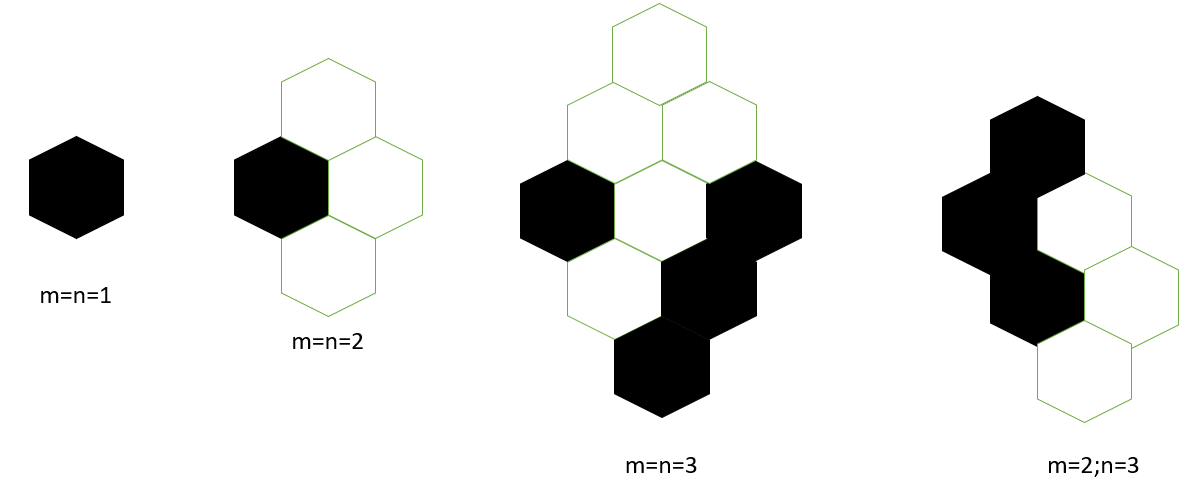
\includegraphics[scale=0.3]{7}
\caption{Sechseckschachbrett.}\end{center}
\end{figure}
\end{center}

\par\noindent Schauen wir uns hierzu einmal den Graphen an. Da man einen Graphen dehnen und drehen darf ohne seine Eigenschaften zu verändern, bringen wir ihn in eine übersichtlichere Darstellung (Pfeil 2, Abb. 2.8). So bekommen wir eine andere Perspektive auf die Figur, die es uns ermöglicht die Figur als \glqq Quadrat\grqq~zu sehen: 
\





\begin{center}
\vspace{-1.5em}
\begin{figure}[H]\label{bild8}
\begin{center}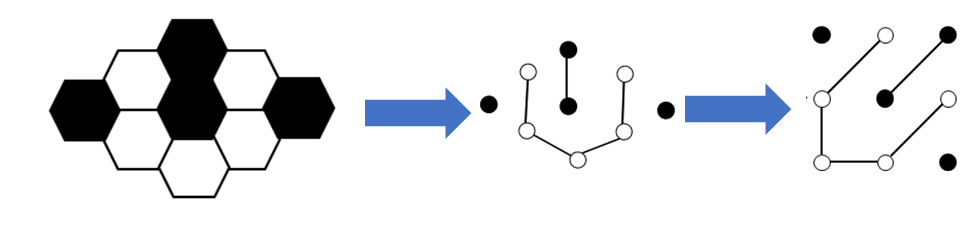
\includegraphics[scale=0.6]{8.png}
\caption{Waben $m=n=3$.}\end{center}
\end{figure}
\end{center}
Setzen wir nun die Angaben in unsere Formel ein. Zuerst also wieder $P=m\cdot n.$
\par\medskip\noindent
Der Erwartungswert der Linien ist wieder die Anzahl aller möglichen Linien multipliziert mit der Wahrscheinlichkeit, dass so eine Linie existiert. Hierbei betrachten wir zuerst die senkrechten und waagrechten Linien. Das sind wie zuvor
$(m-1)n+(n-1)m.$
Nun kommen noch die Diagonalen dazu und zwar $(m-1)(n-1).$
$$\Rightarrow L=(m-1)n+(n-1)m+(m-1)(n-1)$$
$Q$ bezeichnet nun nicht mehr die Anzahl der Quadrate, da wir kleinere Untereinheiten bilden können, nämlich die beiden Dreiecke eines jeden Quadrats. Wir löschen hierbei bei den linken oberen Dreiecken die Diagonale und bei den rechten unteren Dreiecken die rechte Kante, um wieder nichts doppelt zu löschen. Die Anzahl der Dreiecke (also der gewonnenen Kanten) lässt sich dann mit der Formel

$$Q=2(m-1)\cdot(n-1)$$
berechnen. Die Wahrscheinlichkeit für ein gleichfarbiges Dreieck ist nun $\frac{1}{4}=\frac{2}{2^3}$, da an einem Dreieck nur drei Punkte beteiligt sind.\par\noindent

\noindent Fügen wir nun diese Terme zusammen, erhalten wir \small
\begin{align*}
E(G)&\geq mn-\frac{1}{2} [(m-1)n+(n-1)m+(m-1)\cdot(n-1)]+\frac{1}{4} [2(m-1)\cdot(n-1)]=\frac{1}{2} n+\frac{1}{2} m
\end{align*}
\normalsize
\noindent Für mehrere Farben ersetzen wir wieder $\frac{1}{2}$ durch $\frac{1}{F}$, die $\frac{1}{4}$ allerdings durch $\frac{1}{F^2}=\frac{F}{F^3}$, was wieder an den Dreiecken liegt.
Dann ergibt sich:
\begin{align*}
E(G)&\geq mn-\frac{1}{F} [(m-1)n+(n-1)m+(m-1)\cdot(n-1)]+\frac{1}{F^2} [2(m-1)\cdot(n-1)]\\
&=
\left(1-\frac{3}{F}+\frac{2}{F^2}\right)mn+\left(\frac{2}{F}-\frac{2}{F^2}\right)(n+m)+ \left(\frac{2}{F^2} -\frac{1}{F}\right)
\end{align*} 



\section{Mehrere Dimensionen und bessere Abschätzungen}
\subsection{Verallgemeinerung auf \texorpdfstring{$d$}{d} Dimensionen}
In Kapitel 2.3 haben wir uns bereits angeschaut was passiert, wenn man das Schachbrett in einer höheren Dimension als $2$ betrachtet. Dies wollen wir nun mit Hilfe einer Variablen $d$ weiter verallgemeinern. Wir betrachten der Einfachheit halber nur Hyperwürfel, wo alle Seitenlängen gleichlang sind.\\
Erinnern wir uns an unsere Formel:
$$E(G)\geq P-E(L)+E(Q)$$
Die Anzahl der Punkte ist immer das Produkt aus allen Seitenlängen. Bei einem Würfel mit $d$ Dimensionen mit der Seitenlänge $n$ also $n^{d}$.
Berechnen wir nun $L$. Es gibt in jede Raumrichtung $n^{d-1}$ zusammenhängende, parallele und gerade Pfade, da beispielsweise in der Draufsicht entlang dieser Raumrichtung von jedem Punkt der vordersten Hyperebene (vgl. \cite{hyper}) aus ein solcher Pfad nach hinten geht. 
\begin{center}
\begin{figure}[H]\label{Dimension D}
\begin{center}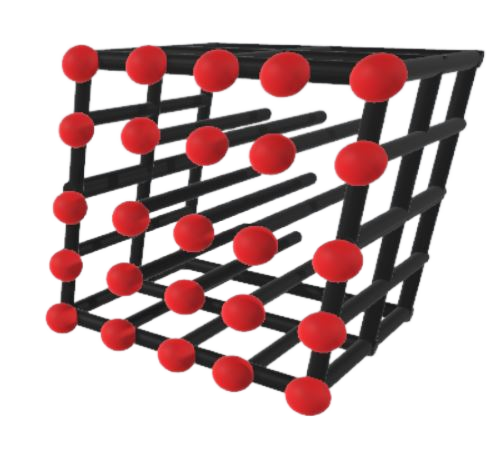
\includegraphics[scale=0.2]{13.png}
\caption{Pfade nach hinten.}\end{center}
\end{figure}
\end{center}
Da es aber $n^{d-1}$ Punkte in dieser vordersten Hyperebene gibt, gehen auch $n^{d-1}$ Pfade nach hinten. Diese Pfade haben eine Länge von $n-1$ Kanten, da jedem Punkt auf diesem Pfad eine Kante zugeordnet ist, außer dem ganz hinten.\\
Die Anzahl der Kanten berechnet sich also wie folgt:

$$L=d\cdot n^{d-1}\cdot (n-1)=d\cdot (n^{d}-n^{d-1})$$
Kommen wir nun zu den Quadraten:\\
$Q$ ist weiterhin die Anzahl der Quadrate allgemein.
Pro zwei fester Raumrichtungen, gibt es nun $n^{d-2}$ zweidimensionale, parallele Flächen.
\begin{center}
\begin{figure}[H]\label{flaechen}
\begin{center}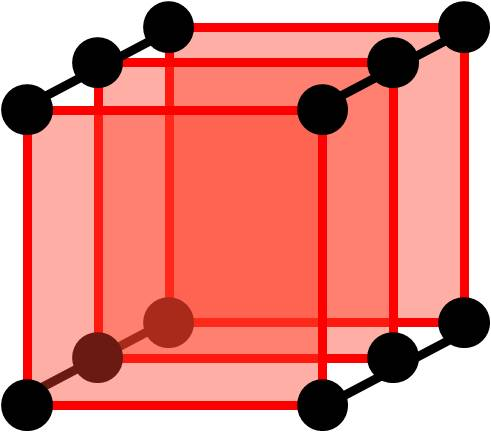
\includegraphics[scale=0.6]{Flaechen}
\caption{Flächenanordnung.}\end{center}
\end{figure}
\end{center}
Da es innerhalb einer solchen Fläche $(n-1)\cdot(n-1)$ Quadrate gibt, ergibt sich für die Anzahl der Quadrate also $n^{d-2}(n-1)^{2},$ wenn man zwei Richtungen (z.B $x$ und $z$) vorgibt. Nun bestimmen wir noch die Anzahl der Kombinationen von Raumrichtungen. Dafür wählen wir immer zwei aus $d$ aus. Wie viele Möglichkeiten es dafür gibt, berechnet man mit dem Binomialkoeffizienten (vgl. \cite{binom}) $$\binom{d}{2}=\dfrac{d\cdot(d-1)}{2}$$ Dementsprechend ist die Anzahl aller Quadrate: $$Q=\dfrac{d\cdot(d-1)}{2}\cdot n^{d-2}\cdot(n-1)^{2}$$
Wie in Kapitel 2.3 beschrieben kann man aber nicht aus allen Quadraten in einem Körper eine Kante löschen, da man sonst eventuell Kanten mehrfach löscht. Deshalb führen wir die neue Variable der sozusagen \glqq unabhängigen\grqq~ Quadrate $Q^*$ ein.
In der dritten Dimension haben wir nur Quadrate betrachtet, die in $xz$- oder $yz$-Richtung liegen. Die Kanten in $z$-Richtungen haben wir immer als Grundgerüst behalten und eine der anderen beiden gelöscht. So gehörte jede Kante, die eventuell gelöscht wird, nur zu einem Quadrat.

Analog halten wir auch in höheren Dimensionen eine Dimension fest und betrachten nur Quadrate, in denen diese eine feste Richtung $d_i$ (z.B. $x,y,z ...$) vorkommt. In all diesen Quadraten gibt es zwei Kanten in $d_i$-Richtung und zwei in eine andere Richtung. Wir löschen hierbei nie die in $d_i$-Richtung, sondern immer eine der anderen, die wir dadurch eindeutig festlegen, dass ihre beiden Punkte eine kleinere $d_i$-Position besitzen.
\begin{center}
\begin{figure}[H]\label{dimens}
\begin{center}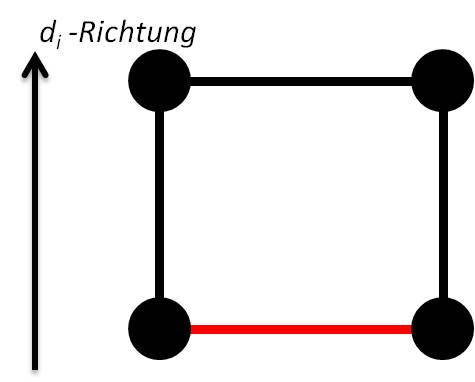
\includegraphics[scale=0.7]{Kante}
\caption{Kantenzuordnung.}\end{center}
\end{figure}
\end{center}So können wir wieder Kanten eindeutig zu einem Quadrat zuordnen, aus welchem wir sie ggf. löschen. Nachdem eine Dimension nun fest ist, bleiben also für die zweite Richtung alle $(d-1)$ anderen Dimensionen übrig. Für unabhängige Quadrate sind also gerade noch $(d-1)$ Kombinationen von Raumrichtungen zulässig. Somit gilt $$Q^*=(d-1)\cdot n^{d-2}\cdot(n-1)^{2}$$
Alle Wahrscheinlichkeiten bleiben (bei $F=2$) gleich, da sie unabhängig von der Dimension sind.
Formen wir nun also unseren Term um.
\begin{align*}
  E(G)&\geq P-E(L)+E(Q^*)\\
  &=n^{d}-\dfrac{1}{2}d\cdot(n^{d}-n^{d-1})+\dfrac{1}{8}(d-1)n^{d-2}\cdot(n-1^{2})\\
&=\left(1-\dfrac{d}{2}+\dfrac{d-1}{8}\right)\cdot n^d+\left(\dfrac{d}{2}-\dfrac{d-1}{4}\right)\cdot n^{d-1}+\dfrac{d-1}{8}n^{d-2}
\end{align*}
Schauen wir uns nun die Wahrscheinlichkeiten in mehreren Farben an.
Wir ersetzen wieder $\frac{1}{2}$ durch $\frac{1}{F}$ und $\frac{1}{8}$ durch $\frac{1}{F^{3}}$ und erhalten
\begin{align*}
    E(G)&\geq n^{d}-\dfrac{1}{F}d\cdot(n^{d}-n^{d-1})+\dfrac{1}{F^3}(d-1)\cdot n^{d-2}\cdot(n-1^{2})\\
    &=\left(1-\dfrac{d}{F}+\dfrac{d-1}{F^3}\right)\cdot n^d+\left(\dfrac{d}{F}-\dfrac{2(d-1)}{F^3}\right)\cdot n^{d-1}+\dfrac{d-1}{F^3}n^{d-2}
\end{align*}
\noindent Wie schon in drei Dimensionen liefert dieser Formel für wenige Farben oft einen negativen Wert und ist somit wenig hilfreich. Eine nützliche Formel entsteht erst, wenn der erste Teil größer gleich 0 ist, dies ist zum Beispiel garantiert, falls
$$ 1-\dfrac{d}{F}\geq 0$$ wahr ist. Daraus folgt, dass die Bedingung der Formel sinnvoll ist, wenn $F\geq d$ gilt.
Für $F<d$ müssen wir uns also eine andere Möglichkeit überlegen, um eine Abschätzung zu erhalten.

\subsection{Lonely Point Methode}
Um eine Abschätzung für hohe Dimensionen und wenig Farben zu erzielen, überlegen wir uns eine Methode, die zwar im Fall $F\geq d$ mit unserer Gebietsabschätzung nicht mithalten kann, dafür aber \textbf{immer} einen positiven Wert garantiert.\\
Hierbei nennen wir Punkte einsam, wenn sie keine Nachbarn der gleichen Farbe haben. Die einsamen Punkte bilden also gerade die Gebiete der Größe 1.
\begin{center}
\begin{figure}[H]\label{lonely}
\begin{center}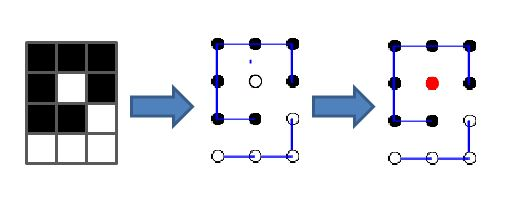
\includegraphics[scale=1]{Lonely.JPG}
\caption{Einsame Punkte sind immer ein Gebiet.}\end{center}
\end{figure}
\end{center}
Diese Zahl (nennen wir sie $G_1$) ist natürlich geringer als die Anzahl aller Gebiete. (Gleichheit herrscht zum Beispiel im Fall des normal gefärbten Schachbretts, wo jedes Feld einsam ist.)
Wir berechnen im nächsten Schritt für jeden Punkt die Wahrscheinlichkeit, dass er einsam ist. Hierbei gehen wir nun zunächst von einem Punkt in der Mitte des Körpers aus (Randpunkte haben schließlich weniger Nachbarn und sind daher in der Abschätzung sogar besser). Im Allgemeinen hat jeder Punkt also (höchstens) $2d$ Nachbarn, da in jeder Dimension zwei dazu kommen. Also ist die Wahrscheinlichkeit, dass ein Punkt einsam ist größer als $\left(\frac{1}{2}\right)^{2d},$
für mehrere Farben dann dementsprechend $\left(\frac{F-1}{F}\right)^{2d}.$
Anschließend multiplizieren wir mit der Anzahl aller Punkte $n^d$. Aufgrund des vorher beschriebenen Zusammenhangs zwischen einsamen Punkten und  Gebieten lässt sich so eine Abschätzung berechnen:
$$E(G)\geq E(G_1)\geq \left(\frac{1}{2}\right)^{2d}n^d=\left(\frac{n}{4}\right)^d$$
Für den $8 \times 8 \times 8$-Würfel erhält man also beispielsweise:
$$E(G)\geq E(G_1)=\left(\frac{1}{2}\right)^6\cdot8 \cdot 8 \cdot 8=\frac{1}{64}\cdot 8 \cdot 8 \cdot 8=8$$
\subsubsection{Genauere Analyse des \texorpdfstring{$8\times 8\times 8$}{8x8x8}-Würfels}
Ziehen wir die Randpunkte nun doch in Betracht, können wir unsere Formel um einiges verbessern. Dies liegt daran, dass es bei einem so kleinen Würfel verhältnismäßig viele Randpunkte gibt.  Dabei fällt auf, dass Punkte in der Oberfläche einen Nachbarn weniger haben, Kantenpunkte zwei und Ecken sogar drei. Damit verdoppelt (vervierfacht oder verachtfacht) sich die Einsamkeitswahrscheinlichkeit. Wir zählen dies so, indem wir in der Rechnung einfach die Punkte entsprechend mehrfach zählen. Nun hat ein $8\times 8 \times 8$-Würfel 8 Eckpunkte und 12 Kanten auf denen je 6 Punkte keine Ecken sind, also 72 Kantenpunkte. Es gibt $6 \cdot 6 \cdot 6$ innere Punkte Also $8^3-6^3$ äußere Punkte. Nun ziehen wir die Kanten- und Eckpunkte ab und erhalten $296-72-8=216$ Flächenpunkte. Nun verbessern wir anhand dessen unsere Abschätzung:
$$E(G)\geq \frac{1}{64}(1\cdot 216+2 \cdot 216+4 \cdot 72+8 \cdot 8)=\dfrac{1000}{64}=\dfrac{125}{8}=15,625$$
Wir werden auf dem Wettbewerb einen sehr schönen Beweis dafür liefern, warum sogar allgemein gilt (für 3 Dimensionen, und Seitenlänge $n$), dass
$$E(G_1)=\left(\dfrac{n+2}{4}\right)^d$$
Man beachte, dass hier tatsächlich Gleichheit gilt, da sich die Anzahl an einsamen Punkte exakt berechnen lassen.

\section{Programmierung}
\subsection{Einführung}
Da wir wissen wollten, wie gut unsere Abschätzungen sind, haben wir ein Programm geschrieben, das eine vorgegebene Zahl an zufälligen Schachbrettern erstellt, jeweils die Gebiete zählt und uns dann den Erwartungswert ausrechnet. Hierfür haben uns unsere Betreuer SciLab empfohlen und mit uns erarbeitet (vgl. \cite{scilab}) -- eine kostenlose Alternative zu MatLab, welche ebenfalls auf Zahlentabellen (mathematisch: Matrizen) basiert
und daher sehr gut für unsere Rechnungen geeignet ist.
\subsection{Warum nur Simulationen und nicht direkt alle Fälle untersuchen?}
Wir haben daran gedacht, einen Algorithmus zu entwickeln, der alle möglichen Fälle zählt, die es bei einem $8\times 8$-Schachbrett gibt. Das wären jedoch $2^{64}$ Fälle, somit würde der Computer sehr lange laufen. Nach unseren Hochrechnungen sogar länger, als es das Universum schon gibt. Wir haben jedoch ein Programm geschrieben, das dies für kleine Bretter tut. Man weiß allerdings, dass wenn man immer mehr zufällige Schachbretter generiert, dies eine immer bessere Näherung für unseren Erwartungswert liefert.
\subsection{Programmidee}
Unsere Simulation für das Zählen der Gebiete besteht aus mehreren Unterprogrammen und einem Hauptprogramm, für die genauen Details verweisen wir auf den Code auf der nächsten Seite:
\begin{itemize}
\item  Die Funktionen „coord“ und „numb“ wechseln zwischen verschiedenen Nummerierungen der Matrix hin und her. Einmal koordinatenweise und einmal listenweise. Dies ist nützlich in den späteren Programmteilen.
\item Das Programm „addneighbours“ fügt zu einer gewissen Anzahl von Startfeldern, die in einem Gebiet liegen, immer weitere Felder desselben Gebietes hinzu. Dabei überprüft es für jedes Feld im bisherigen Gebiet alle vier Nachbarn und fügt sie zu diesem Gebiet hinzu, falls sie dieselbe Farbe haben.
\item 
Das wichtigste Teilprogramm ist „countdom“, das dann tatsächlich alle Gebiete zählt. Dazu starten wir mit einer Liste aller (in diesem Fall 64) Felder (genannt vert) und fangen mit dem ersten an, dann fügen wir mit „addneighbours“ solange alle Nachbarn hinzu, bis keine neuen mehr dazukommen. So haben wir unser erstes Gebiet gefunden. Die Felder von diesem Gebiet löschen wir dann aus unserer Liste und erhöhen den Gebietszähler um eins. Dies machen wir solange, bis die Liste leer ist und wir alle Gebiete gefunden haben.
\item 
Schließlich generieren wir im Hauptprogramm eine gewisse Anzahl an Schachbrettern (im Beispiel 500) mit $f$ Farben (im Beispiel 2) und zählen bei all denen die Gebiete. Zum Schluss bilden wir den Durchschnitt, welcher bei genug Simulationen eine gute Näherung für den Erwartungswert ist.
\end{itemize}

\clearpage
\begin{center}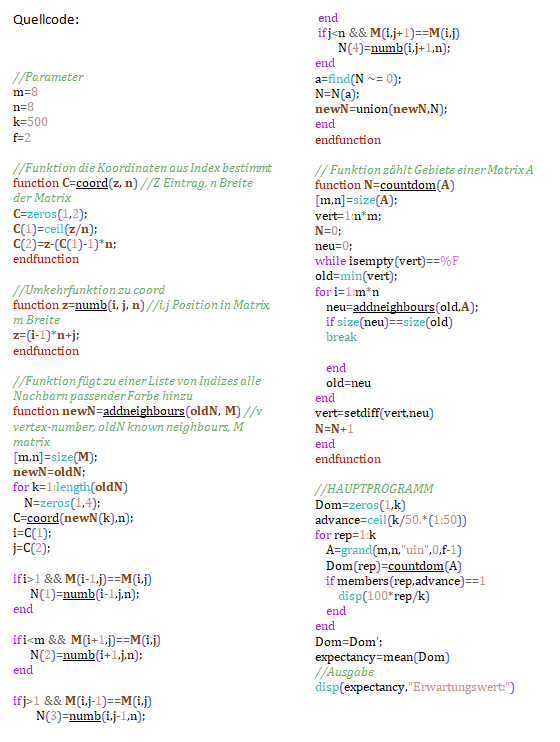
\includegraphics[scale=1.05]{9}
\end{center}
\clearpage
\subsection{Ergebnisse und Fehlerberechnung}
Unsere Betreuer haben uns mathematische Methoden der Statistik gezeigt, um zu berechnen bei wie vielen Versuchen man mit welcher Wahrscheinlichkeit welchen Fehler macht (vgl. \cite{stat}). Ein Konzept ist hierfür die Standardabweichung (vgl. \cite{varianz}). Zum Beispiel ist bekannt, dass man mit rund 95\% Wahrscheinlichkeit nicht mehr als zwei Standardabweichungen daneben liegt, und mit sogar 99,7\% Wahrscheinlichkeit nicht mehr als drei Standardabweichungen (vgl. \cite{normal}). Wollen wir also zum Beispiel, dass unser Erwartungswert mit 99,7\% Wahrscheinlichkeit nicht mehr als $\pm 0,05$ daneben liegt, sollten wir darauf achten, dass unsere Standardabweichung kleiner als $\frac{0,05}{3}=0,0166$ ist.\\
Eine weitere bekannte Formel aus der Statistik besagt, dass sich die Standardabweichung bei $n$ simulierten Versuchen um den Faktor $\sqrt{n}$ verringert. Die Standardabweichung $s$ (bei einem einzelnen Versuch) ist eine abstrakte Größe, welche sich allerdings auch schätzen lässt und in SciLab direkt ausgegeben werden kann. Nun sollte man $k$ also so wählen, dass $\frac{s}{\sqrt{n}}<0,0166$. 
Für das Schachbrett ergibt sich hierbei eine Standardabweichung von rund $3,5$. Dies ist ab knapp $50000$ Versuchen erfüllt. Daher können wir für $k=50000$ mit recht zuverlässigen Werten rechnen, bei dieser Simulation hat sich ein Wert von rund $14,3$ ergeben. Da der Wert unserer theoretischen Abschätzung $14,125$ beträgt, ist unsere Abschätzung für das Schachbrett also relativ gut.
\subsection{Vergleich: Theorie und Praxis}

Nun vergleichen wir auch noch unsere anderen theoretischen Ergebnisse mit den Simulationen aus SciLab. Die kursiven Werte wurden hierbei mit der Lonely-Point-Methode abgeschätzt. In der ersten Zeile vergleichen wir mit dem exakten Wert für ein sehr kleines Schachbrett, darunter betrachten wir unsere Simulationen mit ausreichend Versuchen.
\begin{center}
\begin{tabular}{|c|c|c|c|}
\hline 
Aufgabe & Abschätzung & SciLab-Simulation & Std.-A. ein Versuch \\ 
\hline \hline
$3 \times 4$ Schachbrett (2F) & 4,25 & Exakt! 4,2583 & - \\ 
\hline 
$8 \times 8$ Schachbrett (2F) & 14,125 & 14,3 & 3,5 \\ 
\hline 
$16 \times 16$ Schachbrett (2F) & 44,125 & 45,4 & 6,5 \\ 
\hline 
$8 \times 8$ Torus (2F) & 8 & 9,1 & 3 \\ 
\hline 
$16 \times 16$ Torus(2F) & 32 & 33,8 & 6,4 \\ 
\hline 
$8 \times 8$ Schachbrett (3F) & 28,4815 & 28,5 & 4,1 \\ 
\hline 
$8 \times 8$ Torus (3F) & 23,7073 & 23,8 & 4,4 \\ 
\hline 
$8 \times 8$ Schachbrett (4F) & 36,7656 & 36,8 & 4,3	 \\ 
\hline 
$8 \times 8$ Torus (4F) & 33 & 33,1 & 4,5 \\ 
\hline 
$5 \times 5 \times 5$ Würfel(2F) & \textit{5,36} & 10,0 & 3,2 \\
\hline
$5 \times 5 \times 5$ Würfel(3F) & 30,9259 & 34,6 & 5,8 \\
\hline
$5 \times 5 \times 5$ Würfel(4F) & 52,5 & 54 & 6,2 \\
\hline 
$8 \times 8 \times 8$ Würfel(2F) & \textit{15,625} & 23,2 & 5,32 \\
\hline
$8 \times 8 \times 8$ Würfel(3F) & 93,037 & 113 & 11 \\
\hline
$8 \times 8 \times 8$ Würfel(4F) & 188,25 & 195 & 12,8 \\
\hline
Wabenmuster $5 \times 5$ (2F) & 5 & 5,2 & 1,1 \\ 
\hline 
Wabenmuster $8 \times 8$ (2F) & 8 & 9,0 & 1,7 \\ 
\hline 
Wabenmuster $5 \times 5$ (3F) & 9,88 & 10,0 & 2 \\ 
\hline 
Wabenmuster $8 \times 8$ (3F) & 21,22 & 21,4 & 2,9 \\ 
\hline 
\end{tabular} 
\end{center}
Es fällt hierbei	 auf, dass die simulierten Werte sehr nahe an unseren theoretischen Abschät\-zun\-gen liegen, was bedeutet, dass für die meisten Fälle unsere Methode super ist. Eine größere Abweichung ist beim Torus zu finden, was vermutlich daran liegt, dass dort sehr viele Punkte miteinander verbunden sind und man eigentlich mehr Kanten herauslöschen dürfte, als nur die, die in einem kleinen $2\times 2$-Quadrat auftauchen. Die größte Abweichung findet man bei drei Dimensionen, da unsere theoretische Formel hierbei alle Quadrate in einer Richtung ignoriert.
\section{Ausblick}
Für die Zukunft haben wir noch einige Ideen und Verbesserungsmöglichkeiten:
\begin{itemize}
\item Unseren Algorithmus kann man weiterhin verbessern. Unser Code ist weiterhin noch ziemlich ineffizient und langsam. Wir suchen deshalb hier auf jeden Fall noch bessere Algorithmen, um auch größere Felder und mehr Fälle betrachten zu können. Außerdem sind angepasste Programme für andere Körper (z.B Hyperwürfel) nötig.
\item Weiter kann man auch die Grundformel verbessern. Beispielsweise könnte man noch bessere Formeln finden, die größere Quadrate berücksichtigen oder zum Beispiel die \glqq Lonely Point Methode\grqq~überarbeiten, indem wir z.B. auch Gebiete der Größen $2,3,...$ exakt berechnen.
\item 
Zudem war uns letztes Jahr aufgefallen, dass im echten Hexagon-Schach die Sechsecke anders angeordnet sind, was man ebenfalls gut untersuchen könnte. Dies haben wir uns bereits angeschaut, aber aus Platzgründen nicht aufgeschrieben. Diese Formel lässt sich sicher noch erweitern. 
\end{itemize}
\section{Danksagung}
Erneut bedanken wir uns zunächst bei unseren Mathmatiklehrern Andrea Schaudt, Mattis König und Gerald Baumann für den Spaß, den sie uns die letzten Jahre an der Mathematik vermittelt haben.\par
\noindent Vor allem gilt unser Dank unseren Betreuern am SFZ, David Ploß und Noa Bihlmaier, die uns bei diesem Projekt von Anfang an begleitet haben und uns auch in diesem Jahr uns interressante mathematische Themen und Methoden näher gebracht haben.   \par\noindent Weiter bedanken wir uns bei Helmut Ruf und beim gesamten Schüler\-forschungszentrum für die Räumlichkeiten, das Material und natürlich auch das Angebot im Netz, das uns zur Verfügung gestellt wurde.
\addcontentsline{toc}{section}{Quellenverzeichnis}
\renewcommand{\refname}{Quellenverzeichnis}
\begin{thebibliography}{[99]}

 \bibitem[1]{scilab} Eine Einführung in SciLab/Version 0.997 Alpha/Bruno Pin\c{c}on.
 \bibitem[2]{mathe08} Fundamente der Mathematik 8, unser altes Schulbuch (Stand: Juni 19).
  \bibitem[3]{binom}https://de.wikipedia.org/wiki/Binomialkoeffizient (Stand: Januar 21).
  \bibitem[4]{varianz}https://de.wikipedia.org/wiki/Empirische Varianz \#abgeleitete Begriffe \\ (Stand: November 19).
 \bibitem[5]{graph}https://de.wikipedia.org/wiki/Graphentheorie
(Stand: Oktober 20).
  \bibitem[6]{hyper}https://de.wikipedia.org/wiki/Hyperebene (Stand: Januar 21).
     \bibitem[7]{normal}https://de.wikipedia.org/wiki/Normalverteilung (Stand: November 19).
      \bibitem[8]{torus}https://de.wikipedia.org/wiki/Torus (Stand: Dezember 20).
  \bibitem[9]{stat}https://de.wikipedia.org/wiki/Statistik (Stand: November 19).
 \bibitem[10]{zusammenhangskomponente}https://de.wikipedia.org/wiki/Zusammenhang(Graphentheorie) (Stand: September 19).
  \bibitem[11]{mathe09}Lambacher Schweizer 9 , unser Schulbuch (Stand: Dezember 20).
  
\end{thebibliography}

\end{document}
